\chapter{Contexte et enjeux de la compétition}
    \section{Principe}

        Un modèle génératif de type GAN est présenté, dénoté $\mathcal G$. À l'inverse des GAN classiques généralement utilisés pour générer des images, celui-ci génère des séries temporelles, c'est-à-dire des ensembles ordonnés de données mesurées à intervalles réguliers.

        Le but de la compétition est de trouver les éventuelles faiblesses du GAN en matière de confidentialité, c'est-à-dire s'il est possible de connaître ses données d'entraînement à partir de ses seules données de sortie \textit{(dites données "synthétiques")} $\mathbb S_{Synth}$ dans le cas d'une étude "black-box" ou de ces mêmes données et du modèle lui-même pour une étude "white-box".

        \subsection{\textit{Taxi Trips (2013-2023)} : un dataset public remanié comme donnée d'entrée}
            Le cas considéré ici est tiré d'un dataset disponible publiquement présentant 23 caractéristiques de quelque 200 millions de voyages en taxi dans la ville de Chicago, entre 2013 et 2023.

            Pour la compétition, on extrait de ces données un nouveau dataset comportant les revenus journaliers d'un taxi sur deux semaines. Des opérations de normalisation et de lissage aux extrêmes sont conduites mais non présentées ici.

            Enfin, le dataset présenté aux équipes comporte 1 million de lignes et 7 colonnes
            correspondant aux 7 premiers jours, les revenus de la deuxième semaine étant reportés
            sur
            une nouvelle ligne.
        \subsection{Objectifs et scoring}
            Les équipes se voient confier 4 tâches $T_i, i\in \left[1;4\right]$ dont la particularité est expliquée plus bas. Pour chacune de ces 4 tâches, 100 lignes issues des deux datasets publics $\mathbb{S}_{Pub_{T_1, T_2}}$ et $\mathbb{S}_{Pub_{T_3, T_4}}$, sont regroupées dans un ensemble "cible" que l'on appellera $\mathbb{C}_i, i\in\left[1;4\right]$.

            L'objectif de l'équipe est de déterminer si chaque ligne appartient effectivement
aux datasets d'entraînement $\mathbb{S}_{Pri_{T_i}}$ de $\mathbb G$.

            Le score de chaque tâche est basée sur la différence entre le taux de vrais et de faux positifs, la formule complète étant détaillée dans \cite{snake_strikes_back}.
            \begin{equation}\label{Eq:scoring}
                \mathtt S_{T_i} = \tau_{tp} - \tau_{fp}
            \end{equation}
            \myequations{Formule simplifiée du scoring de la compétition}
    \newpage\section{Particularités de chacune des 4 tâches}
        \subsection{Taille de l'échantillon d'entraînement}
            Le nombre de lignes varie d'un facteur 10 entre les tâches 1-3 et 2-4. Ainsi :
            \begin{itemize}
                \item $\mathbb{S}_{Pri_1}$ et $\mathbb{S}_{Pri_3}$ contiennent 10000 lignes
                \item $\mathbb{S}_{Pri_2}$ et $\mathbb{S}_{Pri_4}$ contiennent 1000 lignes
            \end{itemize}
        \subsection{Connaissance \textit{a priori} des données d'entraînement}
            Les lignes de $\mathbb{S}_{Pri_1}$ et $\mathbb{S}_{Pri_2}$ sont des copies exactes des lignes de $\mathbb{S}_{Pub_{1 | 2}}$.

            Les tâches 3 et 4 sont beaucoup plus subtiles, car les lignes de $\mathbb{S}_{Pri_3}$ et $\mathbb{S}_{Pri_4}$ ne correspondent pas exactement à celles de $\mathbb{S}_{Pub_{3 | 4}}$. Chaque ligne est en fait une concaténation des quatre premiers jours d'une ligne de $\mathbb{S}_{Pub_{3 | 4}}$ et de trois jours n'appartenant pas à ce dataset, et par conséquent hors de la connaissance de l'attaquant.

        \begin{figure}[H]
            \centering
            \subfloat[Pour $\mathbb{S}_{Pub_{1 | 2}}$]{\fbox{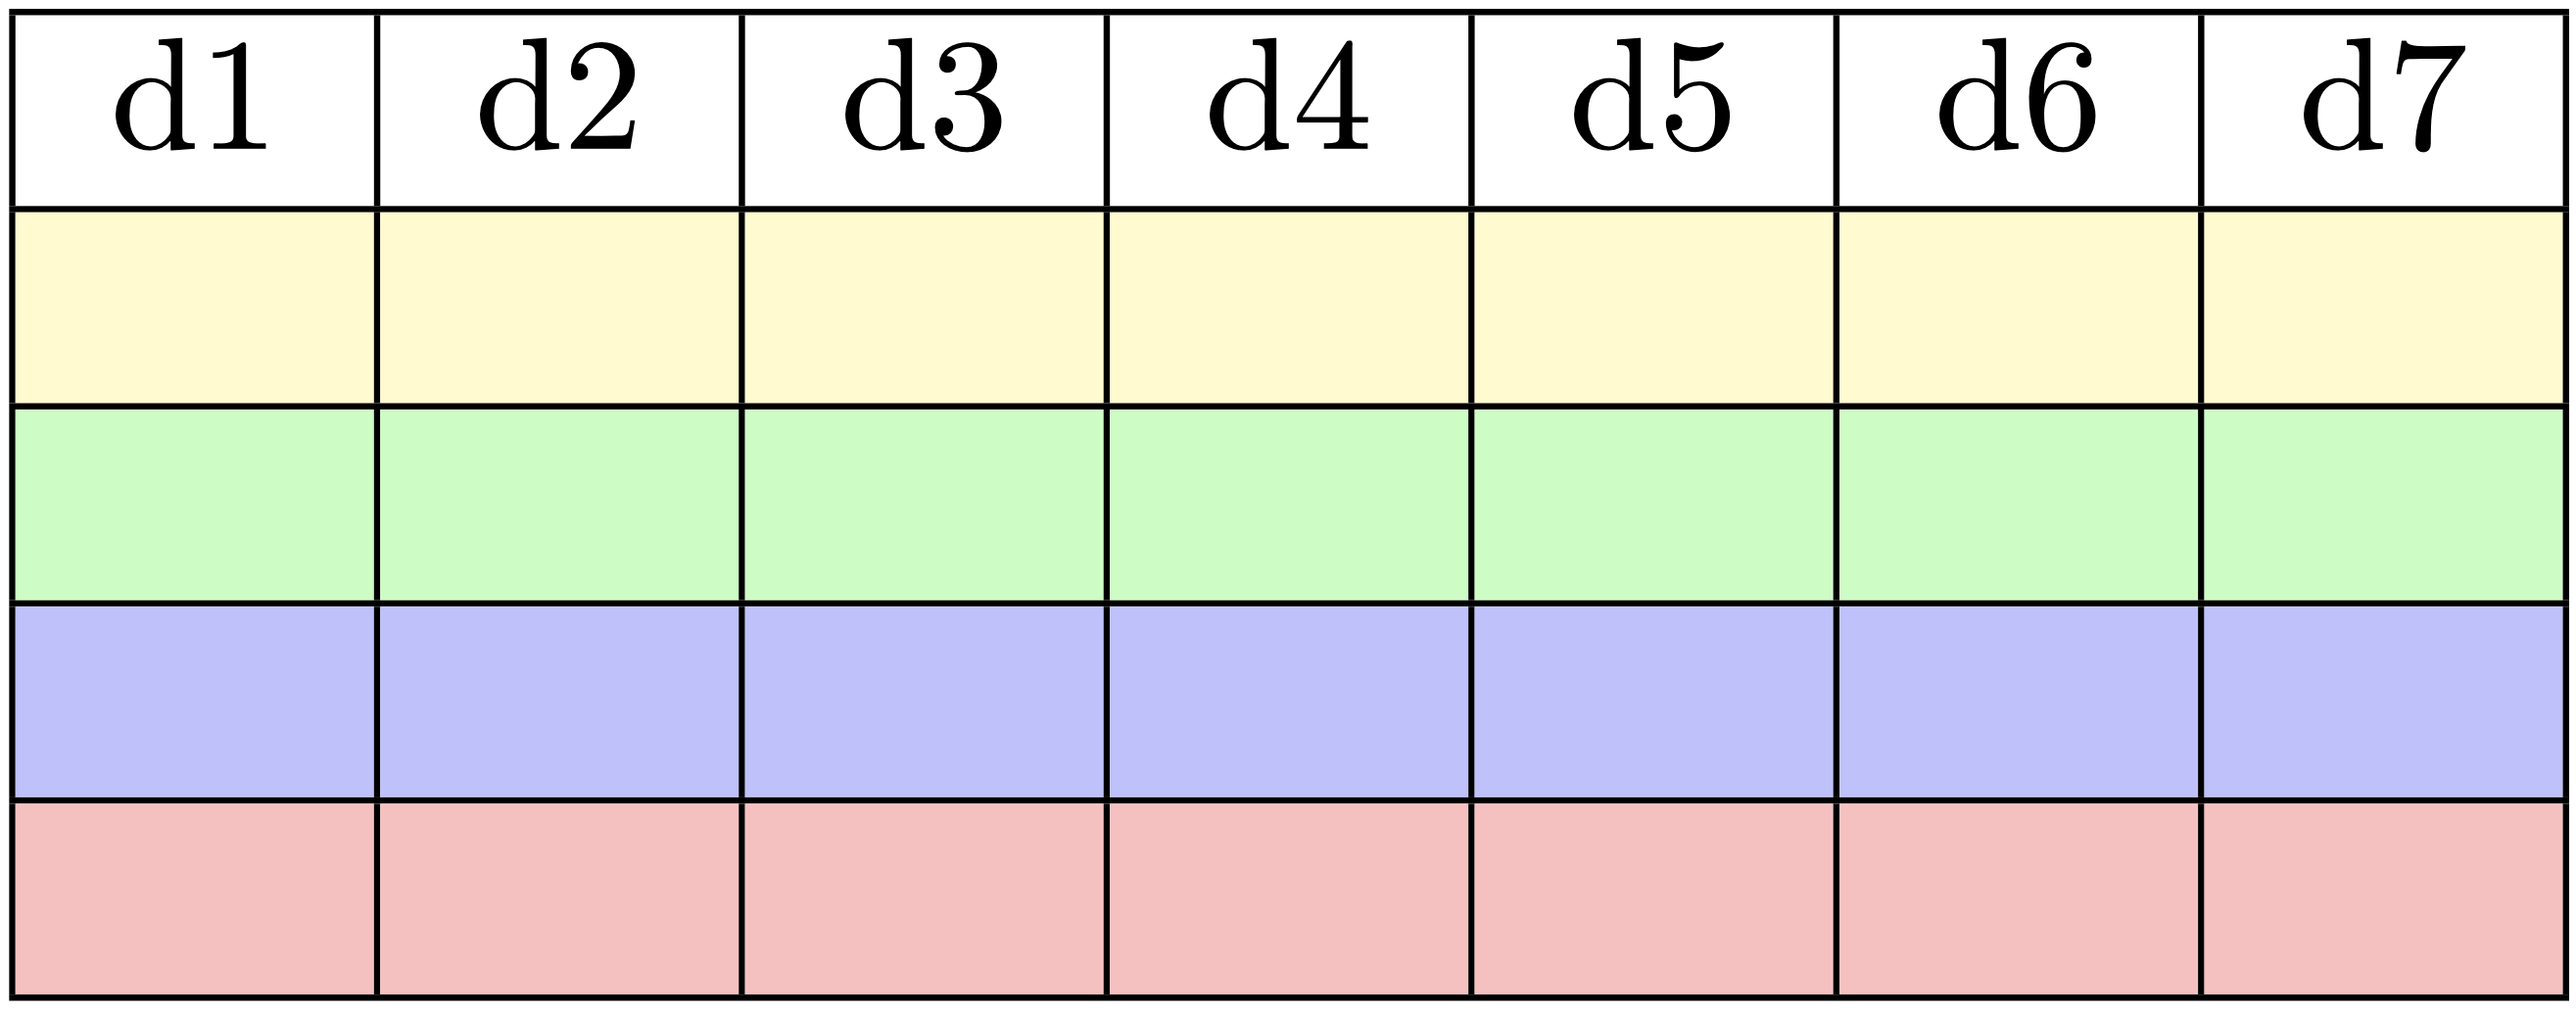
\includegraphics[width = 0.4\textwidth]{figures/Resultats/fromPaper/publicDS_12}}}\qquad
            ~ %espace entre deux images sur une même ligne
            \subfloat[Pour $\mathbb{S}_{Pri_{1,2}}$]{\fbox{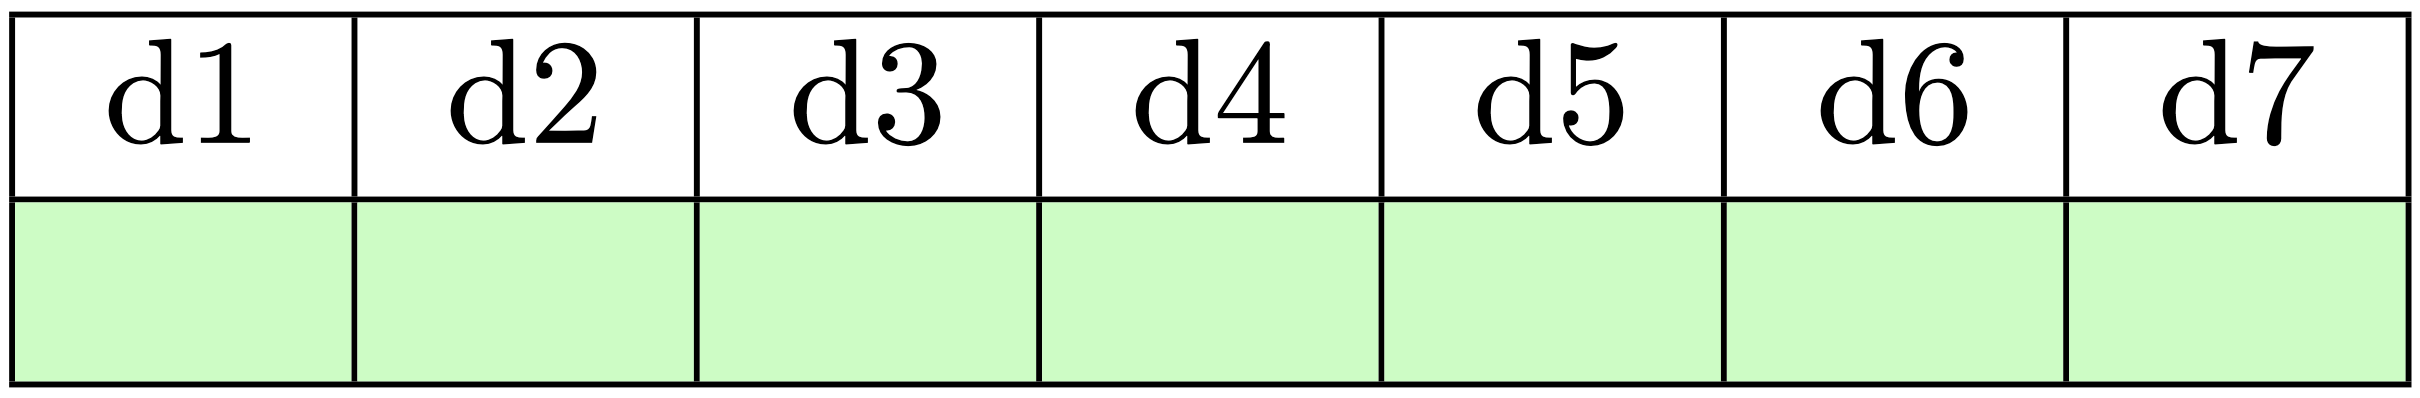
\includegraphics[width = 0.4\textwidth]{figures/Resultats/fromPaper/privateDS_12}}}\qquad
            \subfloat[Pour $\mathbb{S}_{Pub_{3 | 4}}$]{\fbox{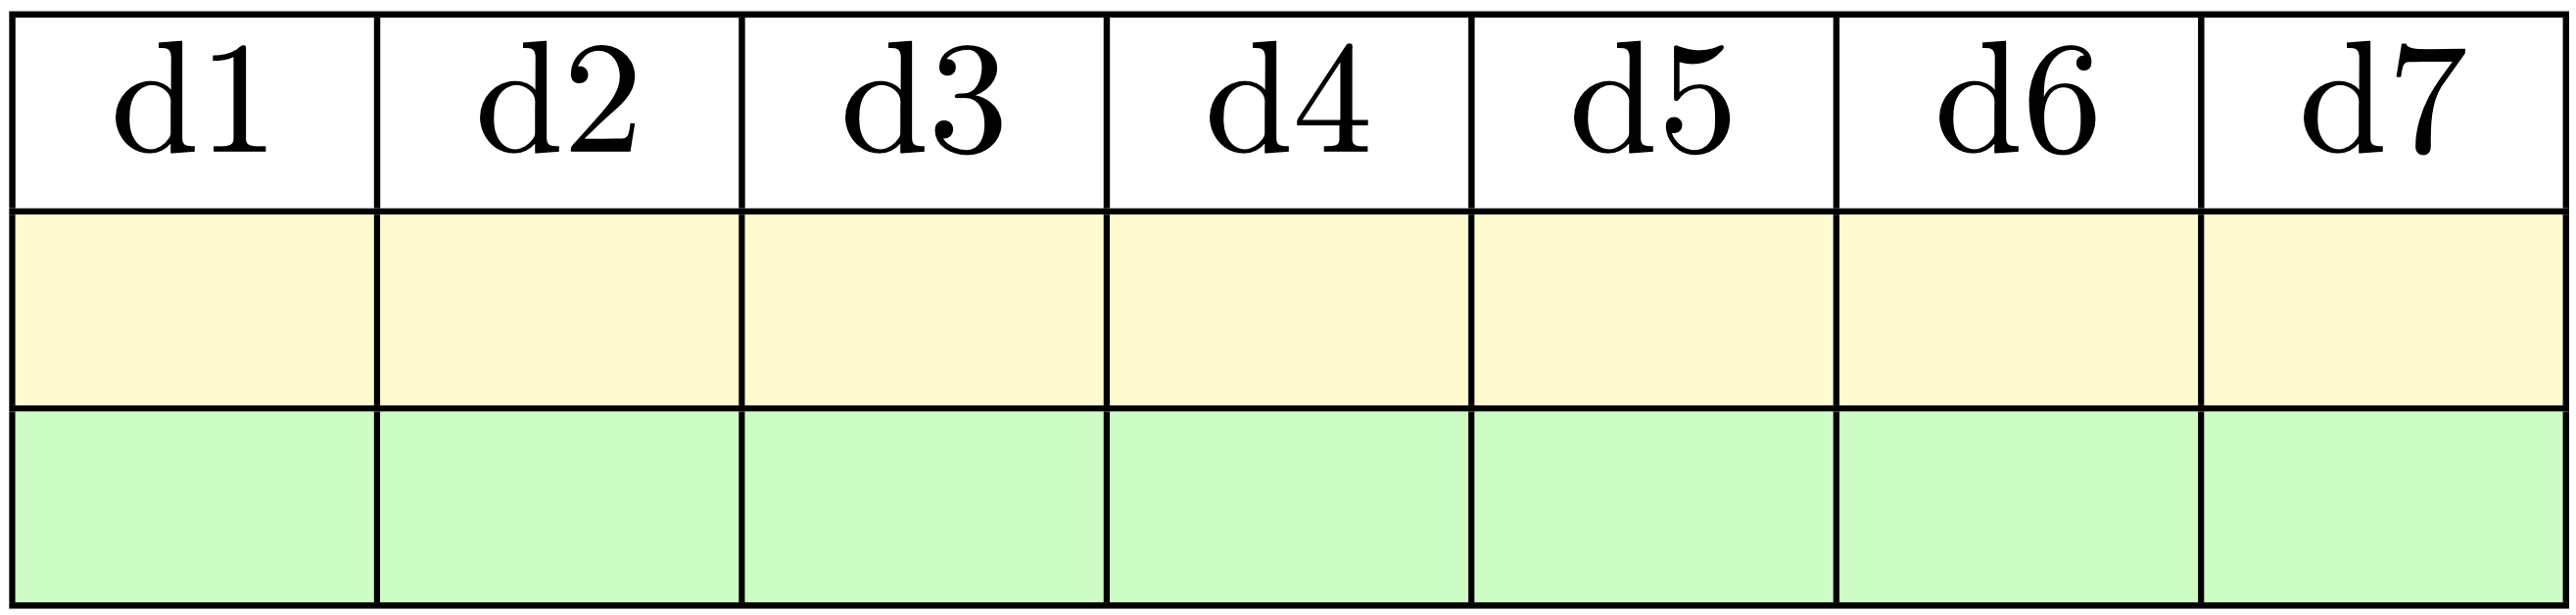
\includegraphics[width = 0.4\textwidth]{figures/Resultats/fromPaper/publicDS_34}}}\qquad
            ~ %espace entre deux images sur une même ligne
            \subfloat[Pour $\mathbb{S}_{Pri_{3,4}}$]{\fbox{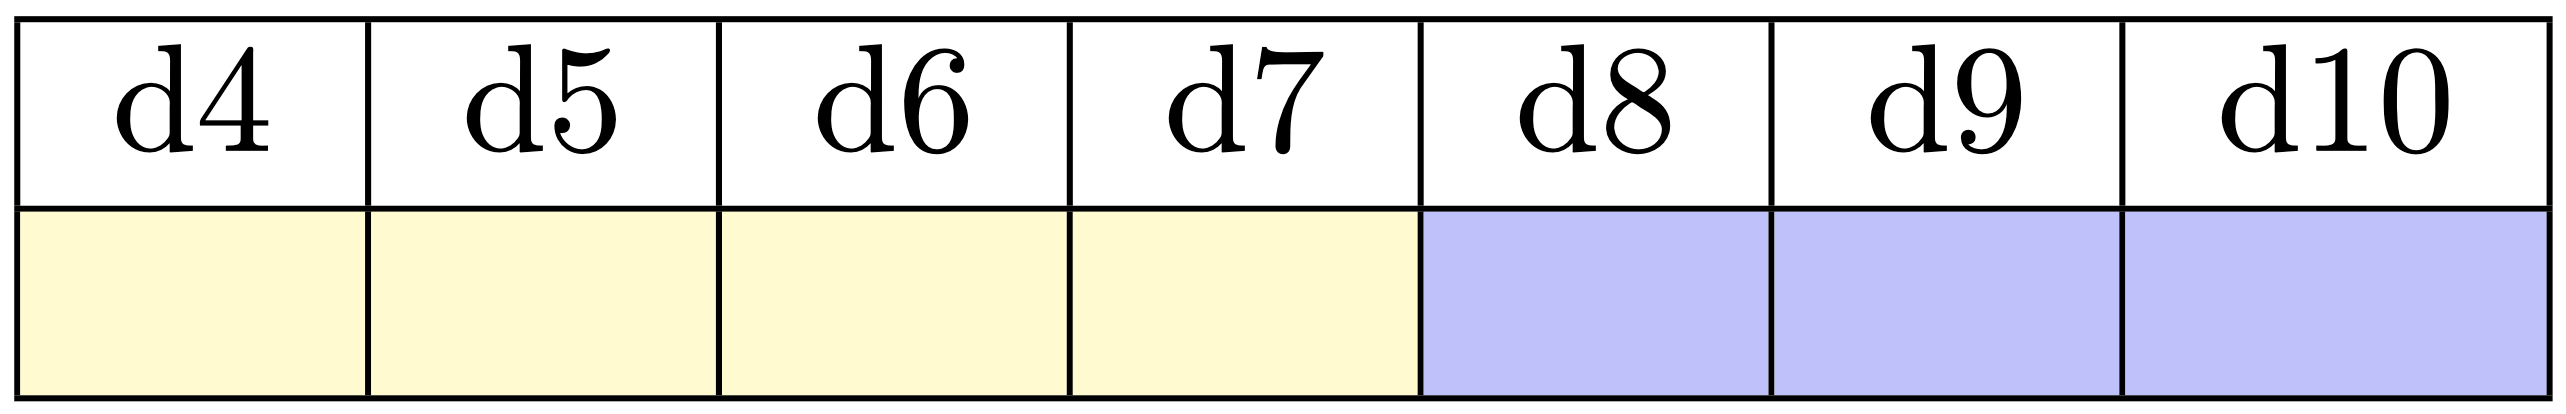
\includegraphics[width = 0.4\textwidth]{figures/Resultats/fromPaper/privateDS34}}}\qquad
            \caption{Exemples de lignes de $\mathbb{S}_{Pub_{1 | 2}}$, $\mathbb{S}_{Pub_{3 | 4}}$ et  $\mathbb{S}_{Pri_i}$}
        \end{figure}


